\chapter{Implementation}

In this thesis I aim to create an LSM-structured implementation of R-trees, which in turn will be write-optimized. To be able to handle a high workload of write operations without compromising query performance, bulk-insertion techniques such as GBI\cite{GBI} and Seeded Clustering\cite{SeededClustering} \textbf{Må finne ut her hva du skal bruke} will be used to make sure that the index structure is not degraded too much. In addition, the use of such techniques will hopefully also generate better storage utilisation which is needed to avoid unnecessary search operations. I have chosen to call my implementation a \emph{Rectangle Structured Merge Tree} or RSM-Tree.

\section{Overview}
In order to implement an R-tree index, while having a LSM-tree structure there are some important aspects to take into consideration. The first is the ordering of the data, as R-trees are used for multi-dimensional data, while LSM-trees are not. In order to do this, the use of ordering techniques are needed, such as Z-order or Hilbert curves. In my implementation, the main ordering technique will be **input here**, but both curves might be tested. Another important aspect is how to merge the data from the upper levels to the lower levels. To do this I have chosen to use bulk-insertion methods which looks at loading smaller R-trees into larger ones. By doing this, the costful operation of creating R-trees from scratch will not be needed with every merge.\newline

Lastly, the choice of merge policies is important. As inspired from Dostoevsky\cite{Dostoevsky}, I will try different combinations of tiering and leveling policies as explained in Section \ref{Dostoevsky}. This is done in order to tune the write and search performance as needed.  

\section{Structure}
The general structure of the RSM-tree is presented in Figure \ref{fig:RSMTree}. The in-memory component $C_0$ stores each data object in their own MBR, given as $A, B, ..., F$. These are sequentially ordered following the chosen space-filling curve. This is done because it is crucial that the items are sequentially ordered when performing search operations in LSM-trees. In addition to this, a sequential structure is beneficial when merging the data to the lower levels, as will be further explained in Section \ref{RSM-Merging}. In the second level $C_1$, the MBRs will be merged together to create R-trees from scratch, given as $R_2, R_3, R_4, R_5$. The lowest level $C_2$, is structured as the main R-tree, where trees from $C_2$ will be bulk-inserted into the correct positions in the main R-tree.  
\begin{figure}[ht]
     \centering
     \begin{subfigure}{0.45\textwidth}
         \centering
         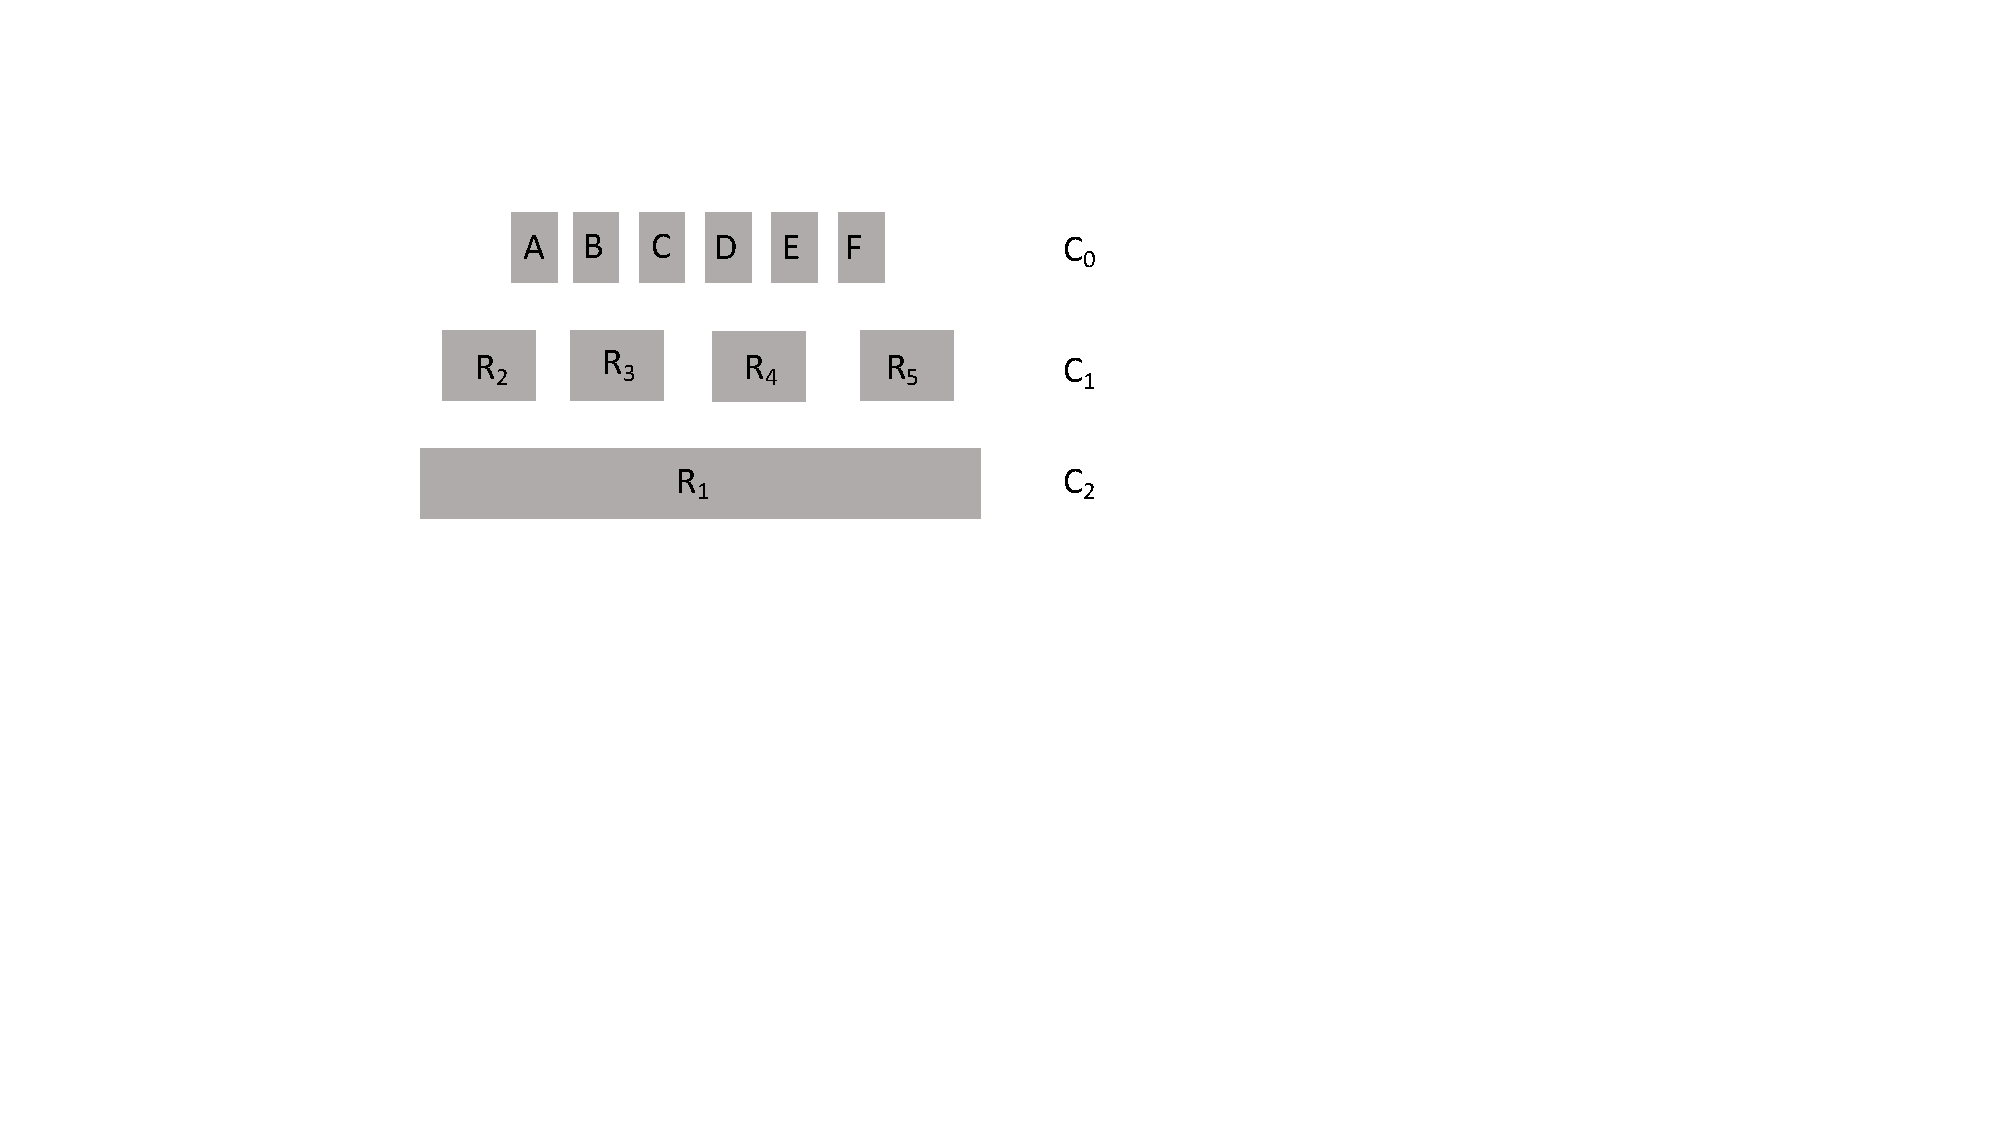
\includegraphics[width=\textwidth]{figures/RSMTree.pdf}
         \caption{RSM-Tree index structure}
     \end{subfigure}
     \hfill
     \begin{subfigure}{0.45\textwidth}
         \centering
         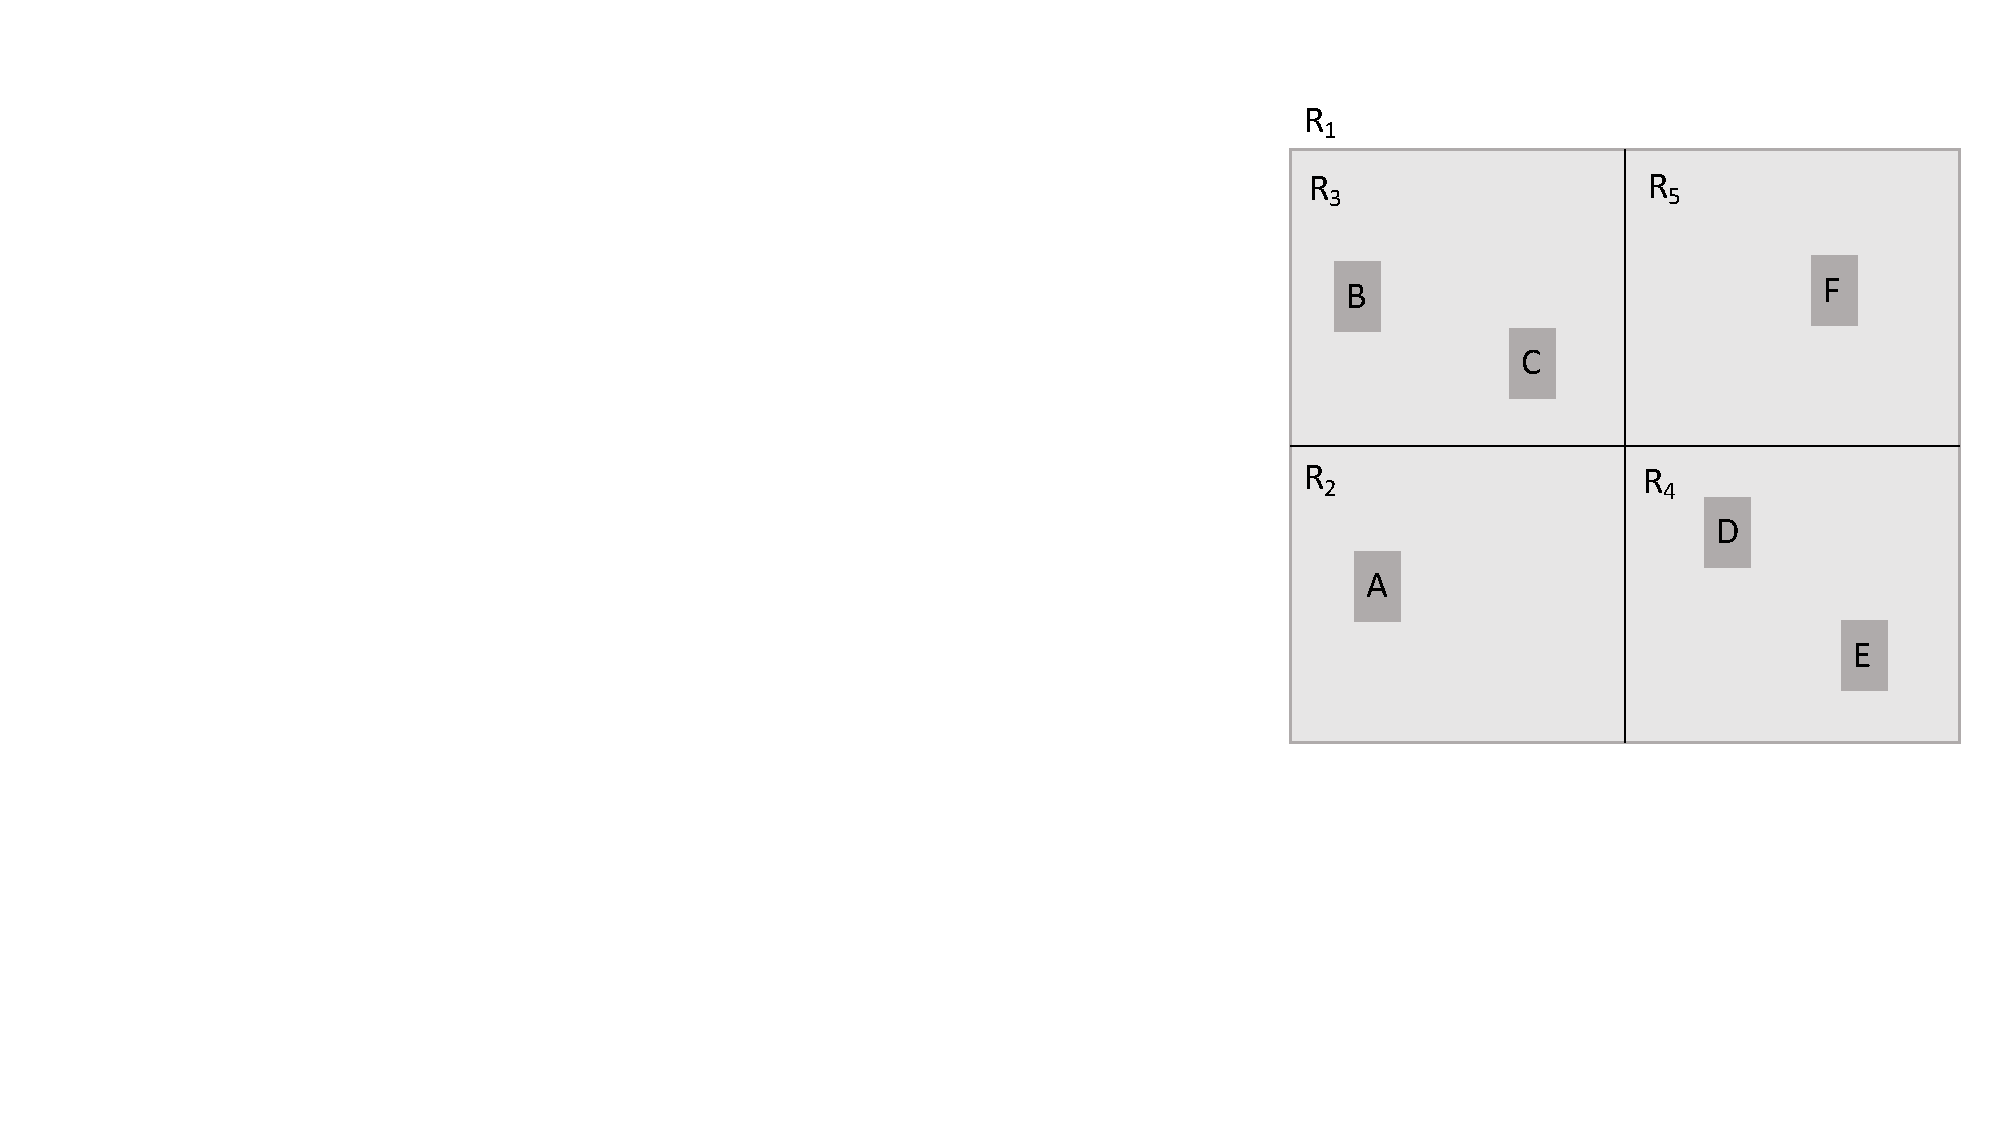
\includegraphics[width=\textwidth]{figures/RSMTree_space.pdf}
         \caption{RSM-Tree space structure}
     \end{subfigure}
        \label{fig:RSMTree}
        \caption{RSM-Tree}
\end{figure}

The nodes in the RSM-tree are structured as shown in Figure \ref{fig:RSMNodes}. \textbf{Her må du finne ut av hvilken space-filling curve du skal ha først..} 

\section{Merging}
\label{RSM-Merging}
The merging technqiue for the RSM-tree is based on both construction of R-trees from scratch, in addition to using bulk-insertion into existing trees. From the in-memory component $C_0$, a portion of $N$ objects are taken at a time to create an R-tree from scratch. This R-tree is then stored at the lower level $C_2$. $N$ is chosen to be a number so that $n$ nodes can be filled with a with a capacity greater than $m$ and smaller than $M$, where $m$ is the minimum number of objects in a node and $M$ is the maximum number of objects. This is done to gurantee that the R-tree structure is valid by avoiding situations where node underflow occurs while still leaving room for additional objects when further merging is done to the lower level. As the objects in $C_0$ are already sequentially ordered by their placements, the trees in $C_1$ are also possible to order. In the optimal scenario, the R-trees in $C_1$ will have no overlap with each other. This can be verified by looking at the overlap between their root nodes. As this might be hard to guarantee in a real-life scenario, this is a challenge that needs to be further investigated when the implementation is created.  \textbf{kanskje noe mer her om hvordan dette skal håndteres, sjekk med SE} \newline

The merging from $C_1$ to the lowest component $C_2$ is done by having an existing R-tree index in the lowest level. When data is ready to be merged from $C_1$, a whole R-tree is bulk-inserted into the main R-tree in $C_3$.

\textbf{Her må det inne noe om hvilken bulk-insertion metode du skal bruke og hvorfor..}